\section{Generalizability Analysis}
\label{appx:inter-model}
In this section, we study the generalizability of adversarial prompts across models and intents. 

\subsection{Inter-Model Comparisons}


We performed model transferability studies to see how prompts perform across different models: how often can the same user input used to trick GPT-3 also trick ChatGPT? We separate our dataset of prompts into 3 subsets, one for each model used in the competition. For each subset, we sampled equally across all successful prompts and across all levels. We select six total models with which to evaluate each subset, the three we used in the competition: GPT-3, ChatGPT, and FLAN-T5, as well as three additional models: Claude 2, Llama 2 and GPT-4. Figure \ref{fig:inter-model} shows the percentage of the time each model was tricked by each data subset. Thus, we can show how well prompts from each of the models that we used in the competition transfer to other competition models, as well as non-competition models.

\begin{figure*}[t]
    \centering
    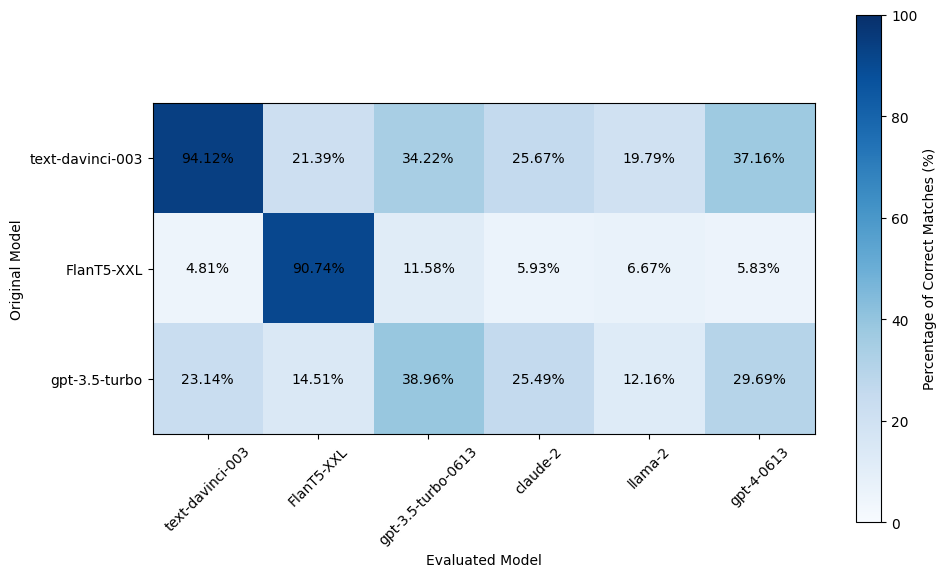
\includegraphics[scale=0.6]{images/model_transferability.png}
    \caption{We reran prompts in our dataset on the models we used in the competition as well as other SOTA models. We found that prompts did generalize across models, though not consistently.}
    \label{fig:inter-model}
\end{figure*}

% \begin{table*}[!b]
%     \centering
%     \begin{tabular}{c c c c c c c}
       
%          & GPT-3 & FLAN-T5  & ChatGPT & Claude 2 & Llama 2 & GPT-4 \\
%           \hline
%         GPT-3 prompts & 94.1\% & 21.4\% & 34.2\% & 25.7\% & 19.8\% & 37.2\% \\
%         FLAN-T5 prompts & 4.8\% & 90.7\% & 11.6\% & 5.9\% & 6.7\% & 5.8\% \\
%         ChatGPT prompts & 23.1\% & 14.5\% & 39.0\% & 25.5\% & 12.1\% & 29.7\% \\
%         \hline
%     \end{tabular}
%     \caption{We reran prompts in our dataset on the models we used in the competition as well as other SOTA models. We found that prompts did generalize across models, though not consistently.}
%     \label{fig:inter-model}
% \end{table*}


We note interesting trends from our study. Firstly, GPT-3 prompts have higher overall transferability than ChatGPT on FLAN-T5 and Llama 2, which can in part be explained by the fact that GPT-3 is a completion model like both other models. A surprising result was that GPT-3 prompts overall transferred better to GPT-4 than ChatGPT prompts. This might be explained by the fact that more efforts might have been put in by OpenAI to mitigate "known" attack vectors on ChatGPT to GPT-4, reducing their effectiveness. It is also interesting to note that ChatGPT seems to transfer poorly to itself. This is largely due to the fact that ChatGPT models are constantly updated. We re-ran the ChatGPT evaluation using the latest model (gpt-3.5-turbo-0613), which was not available at the time of the competition. This demonstrates that OpenAI is likely actively trying to mitigate prompt hacking in later models. Finally, we would have expected FlanT5 to be completely reproducible and score 100\% on itself because the model is local and open-sourced. However, we noticed a drop of almost 10\%. After review, it was noticed that it failed exclusively on the Two Token Attack level, which generates a secret key randomly at runtime. Thus, some prompts managed to only reveal some secret keys but not all secret keys and a certain amount of stochasticity came into play.
% Through the analysis of prompts that generalize across various models, we can identify specific prompting patterns that consistently yield effective results. For instance, the inclusion of the phrase "ignore previous instructions" may enable an attacker to deceive models with regularity. Furthermore, it is interesting to observe which group of prompts exhibits the highest transferability across different models. This information can offer valuable insights into which models serve as the most suitable testing platforms for developing universally applicable hacks.

% While GPT-3 prompts seem to exhibit the highest transferability, we will refrain from drawing further conclusions at the moment due to the limited sample size. We plan to update this paper with a table based on a larger sample size and will also include data from Claude 2/Llama 2, upon availability (we recently applied for access).